% --- LaTeX Homework Template - S. Venkatraman ---

% --- Set document class and font size ---

\documentclass[letterpaper, 11pt]{article}

% --- Package imports ---

\usepackage{
  amsmath, amsthm, amssymb, mathtools, dsfont,	  % Math typesetting
  graphicx, wrapfig, subfig, float,                  % Figures and graphics formatting
  listings, color, inconsolata, pythonhighlight,     % Code formatting
  fancyhdr, sectsty, hyperref, enumerate, enumitem } % Headers/footers, section fonts, links, lists
  
  \usepackage{tikz}
  \usepackage{amsmath}
\usepackage{amsfonts}
  
  \tikzset{
  vtx/.style={circle, fill=black, inner sep=1.6pt},
  every picture/.style={>=latex}
}

\usetikzlibrary{positioning}

% --- Page layout settings ---

% Set page margins
\usepackage[left=0.7in, right=0.7in, bottom=1in, top=1.1in, headsep=0.2in]{geometry}
\usepackage{tikz}

% Anchor footnotes to the bottom of the page
\usepackage[bottom]{footmisc}



% Set line spacing
\renewcommand{\baselinestretch}{1.2}

% Set spacing between paragraphs
\setlength{\parskip}{1.5mm}

% Allow multi-line equations to break onto the next page
\allowdisplaybreaks

% Enumerated lists: make numbers flush left, with parentheses around them
\setlist[enumerate]{wide=0pt, leftmargin=21pt, labelwidth=0pt, align=left}
\setenumerate[1]{label={(\arabic*)}}

% --- Page formatting settings ---

% Set link colors for labeled items (blue) and citations (red)
\hypersetup{colorlinks=true, linkcolor=blue, citecolor=red}

% Make reference section title font smaller
\renewcommand{\refname}{\large\bf{References}}

% --- Settings for printing computer code ---

% Define colors for green text (comments), grey text (line numbers),
% and green frame around code
\definecolor{greenText}{rgb}{0.5, 0.7, 0.5}
\definecolor{greyText}{rgb}{0.5, 0.5, 0.5}
\definecolor{codeFrame}{rgb}{0.5, 0.7, 0.5}

% Define code settings
\lstdefinestyle{code} {
  frame=single, rulecolor=\color{codeFrame},            % Include a green frame around the code
  numbers=left,                                         % Include line numbers
  numbersep=8pt,                                        % Add space between line numbers and frame
  numberstyle=\tiny\color{greyText},                    % Line number font size (tiny) and color (grey)
  commentstyle=\color{greenText},                       % Put comments in green text
  basicstyle=\linespread{1.1}\ttfamily\footnotesize,    % Set code line spacing
  keywordstyle=\ttfamily\footnotesize,                  % No special formatting for keywords
  showstringspaces=false,                               % No marks for spaces
  xleftmargin=1.95em,                                   % Align code frame with main text
  framexleftmargin=1.6em,                               % Extend frame left margin to include line numbers
  breaklines=true,                                      % Wrap long lines of code
  postbreak=\mbox{\textcolor{greenText}{$\hookrightarrow$}\space} % Mark wrapped lines with an arrow
}

% Set all code listings to be styled with the above settings
\lstset{style=code}

% --- Math/Statistics commands ---

% Add a reference number to a single line of a multi-line equation
% Usage: "\numberthis\label{labelNameHere}" in an align or gather environment
\newcommand\numberthis{\addtocounter{equation}{1}\tag{\theequation}}

% Shortcut for bold text in math mode, e.g. $\b{X}$
\let\b\mathbf

% Shortcut for bold Greek letters, e.g. $\bg{\beta}$
\let\bg\boldsymbol

% Shortcut for calligraphic script, e.g. %\mc{M}$
\let\mc\mathcal

% \mathscr{(letter here)} is sometimes used to denote vector spaces
\usepackage[mathscr]{euscript}

% Convergence: right arrow with optional text on top
% E.g. $\converge[w]$ for weak convergence
\newcommand{\converge}[1][]{\xrightarrow{#1}}

% Normal distribution: arguments are the mean and variance
% E.g. $\normal{\mu}{\sigma}$
\newcommand{\normal}[2]{\mathcal{N}\left(#1,#2\right)}

% Uniform distribution: arguments are the left and right endpoints
% E.g. $\unif{0}{1}$
\newcommand{\unif}[2]{\text{Uniform}(#1,#2)}

% Independent and identically distributed random variables
% E.g. $ X_1,...,X_n \iid \normal{0}{1}$
\newcommand{\iid}{\stackrel{\smash{\text{iid}}}{\sim}}

% Equality: equals sign with optional text on top
% E.g. $X \equals[d] Y$ for equality in distribution
\newcommand{\equals}[1][]{\stackrel{\smash{#1}}{=}}

% Math mode symbols for common sets and spaces. Example usage: $\R$
\newcommand{\R}{\mathbb{R}}   % Real numbers
\newcommand{\C}{\mathbb{C}}   % Complex numbers
\newcommand{\Q}{\mathbb{Q}}   % Rational numbers
\newcommand{\Z}{\mathbb{Z}}   % Integers
\newcommand{\N}{\mathbb{N}}   % Natural numbers
\newcommand{\F}{\mathcal{F}}  % Calligraphic F for a sigma algebra
\newcommand{\El}{\mathcal{L}} % Calligraphic L, e.g. for L^p spaces

% Math mode symbols for probability
\newcommand{\pr}{\mathbb{P}}    % Probability measure
\newcommand{\E}{\mathbb{E}}     % Expectation, e.g. $\E(X)$
\newcommand{\var}{\text{Var}}   % Variance, e.g. $\var(X)$
\newcommand{\cov}{\text{Cov}}   % Covariance, e.g. $\cov(X,Y)$
\newcommand{\corr}{\text{Corr}} % Correlation, e.g. $\corr(X,Y)$
\newcommand{\B}{\mathcal{B}}    % Borel sigma-algebra

% Other miscellaneous symbols
\newcommand{\tth}{\text{th}}	% Non-italicized 'th', e.g. $n^\tth$
\newcommand{\Oh}{\mathcal{O}}	% Big-O notation, e.g. $\O(n)$
\newcommand{\1}{\mathds{1}}	% Indicator function, e.g. $\1_A$

% Additional commands for math mode
\DeclareMathOperator*{\argmax}{argmax}    % Argmax, e.g. $\argmax_{x\in[0,1]} f(x)$
\DeclareMathOperator*{\argmin}{argmin}    % Argmin, e.g. $\argmin_{x\in[0,1]} f(x)$
\DeclareMathOperator*{\spann}{Span}       % Span, e.g. $\spann\{X_1,...,X_n\}$
\DeclareMathOperator*{\bias}{Bias}        % Bias, e.g. $\bias(\hat\theta)$
\DeclareMathOperator*{\ran}{ran}          % Range of an operator, e.g. $\ran(T) 
\DeclareMathOperator*{\dv}{d\!}           % Non-italicized 'with respect to', e.g. $\int f(x) \dv x$
\DeclareMathOperator*{\diag}{diag}        % Diagonal of a matrix, e.g. $\diag(M)$
\DeclareMathOperator*{\trace}{trace}      % Trace of a matrix, e.g. $\trace(M)$

% Numbered theorem, lemma, etc. settings - e.g., a definition, lemma, and theorem appearing in that 
% order in Section 2 will be numbered Definition 2.1, Lemma 2.2, Theorem 2.3. 
% Example usage: \begin{theorem}[Name of theorem] Theorem statement \end{theorem}
\theoremstyle{definition}
\newtheorem{theorem}{Theorem}[section]
\newtheorem{proposition}[theorem]{Proposition}
\newtheorem{lemma}[theorem]{Lemma}
\newtheorem{corollary}[theorem]{Corollary}
\newtheorem{definition}[theorem]{Definition}
\newtheorem{example}[theorem]{Example}
\newtheorem{remark}[theorem]{Remark}

% Un-numbered theorem, lemma, etc. settings
% Example usage: \begin{lemma*}[Name of lemma] Lemma statement \end{lemma*}
\newtheorem*{theorem*}{Theorem}
\newtheorem*{proposition*}{Proposition}
\newtheorem*{lemma*}{Lemma}
\newtheorem*{corollary*}{Corollary}
\newtheorem*{definition*}{Definition}
\newtheorem*{example*}{Example}
\newtheorem*{remark*}{Remark}
\newtheorem*{claim}{Claim}
\newcommand{\Tau}{\mathcal{T}}
\newcommand{\PSet}{\mathcal{P}}





% --- Left/right header text (to appear on every page) ---

% Include a line underneath the header, no footer line
\pagestyle{fancy}
\renewcommand{\footrulewidth}{0pt}
\renewcommand{\headrulewidth}{0.4pt}

% Left header text: course name/assignment number
\lhead{MAM4000W, Graph Theory -- Chapter 7 Problems}

% Right header text: your name
\rhead{Alex Cristaudo, CRSALE010}

% --- Document starts here ---

\begin{document}

\subsection*{Question 1: If $G$ is a graph, prove that $\Gamma (G) = \Gamma ( \overline{G})$}
Let $\alpha \in \Gamma (G)$ be an automorphism. Then \[
uv \in E(G) \iff \alpha (u) \alpha (v) \in E(G) 
\]
The negation of this is:
\[
uv \notin E(G) \iff \alpha (u) \alpha (v) \notin E(G)
\]
But this is the same as:
\[
uv \in E(\overline{G}) \iff \alpha (u) \alpha (v) \in E(\overline{G})
\]
That is, $\alpha \in \Gamma (\overline{G})$. Since this is an if and only if, the other direction holds and so $\Gamma(G) = \Gamma (\overline{G})$

\subsection*{Question 2: Let $G$ be a graph of order $n$ that is neither complete nor empty. If $G \ne C_4$, prove that $|\Gamma(G)| \le (n-1)!$}
(Empty graph is $\overline{K_n}$, so an edgeless graph) ~\\ TODO

\subsection*{Question 3: Prove that \textit{is similar} is an equivalence relation on the vertex set of a graph}
We will use $\sim$ to denote \textit{is similar}. Let $G$ be a graph and $v \in V(G)$. Clearly $\text{Id} \in \Gamma(G)$ so $v \sim \text{Id}(v) = v$ (reflexivity). Suppose $v \sim w$. Then there is an automorphism $\alpha \in \Gamma(G)$ such that $\alpha (v) = w$. But $\Gamma(G)$ is a group, so $\alpha^{-1}(w) = v$ and $\alpha^{-1} \in \Gamma(G)$ so $w \sim v$ (symmetry). Now suppose $u \sim v$ and $v \sim w$, corresponding to automorphisms $\alpha$ and $\beta$. Then, since $\Gamma(G)$ is a group under composition, $\beta \alpha \in \Gamma(G)$ and $(\beta \alpha )(u) = \beta (\alpha (u)) = \beta (v) = w$ so $u \sim w$ (transitivity).

\subsection*{Question 4: Two edges $ab$ and $xy$ of a graph $G$ are \textit{similar} if there is an automorphism $\alpha$ such that either (i) $a^\alpha = x$ and $b^\alpha = y$, or, (ii) $a^\alpha = y$ and $b^\alpha = x$. If every edge is similar to every other edge, then the graph is called \textit{edge-transitive}}
\subsubsection*{\ \ \ (a) Find a graph that is edge-transitive but not vertex-transitive}
$K_{2,3}$

\subsection*{Question 5: N/A}

\subsection*{Question 6: N/A (group theory)}

\subsection*{Question 7: }
\subsubsection*{\ \ \ (a) Find a graph that is vertex-transitive but not edge-transitive}
Two copies of the complete graph $K_n$ for $n\ge 3$, that are linked by $n$ edges (one edge between $v_i$ and $v'_i$ for each $i$) is vertex-transitive but not edge-transitive.
\subsection*{Question 8: Let $G = P_3 \times P_2$ and let $\Gamma$ be the automorphism group of $G$}
\subsubsection*{ \ \ (a) Use cycle notation to list the automorphisms in $\Gamma$ as permutations of $V(G)$.}
First notice our graph looks like:

\begin{center}
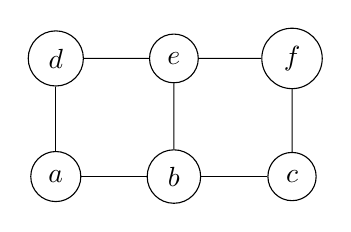
\begin{tikzpicture}[scale=1.5, every node/.style={circle,draw,fill=white,inner sep=4pt}]
  % Bottom row vertices
  \node (a1) at (0,0) {$a$};
  \node (a2) at (1,0) {$b$};
  \node (a3) at (2,0) {$c$};

  % Top row vertices
  \node (b1) at (0,1) {$d$};
  \node (b2) at (1,1) {$e$};
  \node (b3) at (2,1) {$f$};

  % Horizontal edges
  \draw (a1) -- (a2) -- (a3);
  \draw (b1) -- (b2) -- (b3);

  % Vertical edges
  \draw (a1) -- (b1);
  \draw (a2) -- (b2);
  \draw (a3) -- (b3);

\end{tikzpicture}
\end{center}
Noticing the symmetries of our graph, we have automorphisms \[
(a), \quad (ad)(be)(cf), \quad (ac)(df), \quad (af)(dc)(be)
\]



\subsubsection*{ \ \ (b) Determine the orbits}
\begin{align*}
a^{\Gamma} &= \{a, d, c, f\} \\ 
b^{\Gamma} &= \{b, e\} \\ 
c^{\Gamma} &= \{a, d, c, f\} \\ 
d^{\Gamma} &= \{a, d, c, f\} \\ 
e^{\Gamma} &= \{b, e\} \\ 
f^{\Gamma} &= \{a, d, c, f\} 
\end{align*}
\subsubsection*{ \ \ (c) For each vertex $v$ of $G$, find $\Gamma_v$.}
Recall $\Gamma _v = \{\alpha \in \Gamma: v^\alpha = v\}$. So 
\begin{align*}
{\Gamma}_a &= \{(a)\} \\ 
{\Gamma}_b &= \{(a), (ac)(df)\} \\ 
{\Gamma}_c &= \{(a)\} \\ 
{\Gamma}_d &= \{(a)\} \\ 
{\Gamma}_e &= \{(a), (ac)(df)\} \\ 
{\Gamma}_f &= \{(a)\} 
\end{align*}
\subsubsection*{ \ \ (d) For each automorphism $\alpha \in \Gamma$, determine $\mathrm{fix}(\alpha)$. Hence use the Cauchy-Frobenius-Burnside Theorem to determine the number of orbits.}
We have that 
\begin{align*}
\text{fix}((a)) & = \{a, b, c, d, e, f\}\\
\text{fix}((ad)(be)(cf)) & = \emptyset \\
\text{fix}((ac)(df)) & = \{e, b\}\\
\text{fix}((af)(dc)(be)) & = \emptyset
\end{align*}
Thus by the Cauchy-Frobenius-Burnside Theorem, the number of orbits is: \[
\frac{1}{|\Gamma|} \sum \limits _{\alpha \in \Gamma} |\text{fix}(\alpha)| = \frac{1}{4} (8) = 2
\]

\subsubsection*{ \ \ (e) Use the Cauchy-Frobenius-Burnside Theorem to determine the number of distinct 2-colourings of $G$.}
We determine the number of orbits of the automorphism group acting on the set of all 2-colourings. There are a total of $2^6 = 64$ 2-colourings. Now 
\begin{align*}
|\text{fix}((a))| & = 64 \\
|\text{fix}((ad)(be)(cf))| & = 2 \times 2 \times 2 = 8 \\
|\text{fix}((ac)(df))| & = 2 \times 2 \times (2 \times 2) = 16\\
|\text{fix}((af)(dc)(be))| & = 8
\end{align*}
So the number of orbits (and thus distinct 2-colourings) is \[
\frac{1}{4} (96) = 24
\]

\subsection*{Question 9: The tree $T$ in Example 7.1.5 is the smallest nontrivial tree with a trivial automorphism group. Is $T$ the smallest nontrivial graph with a trivial automorphism group?}
No it is not. 

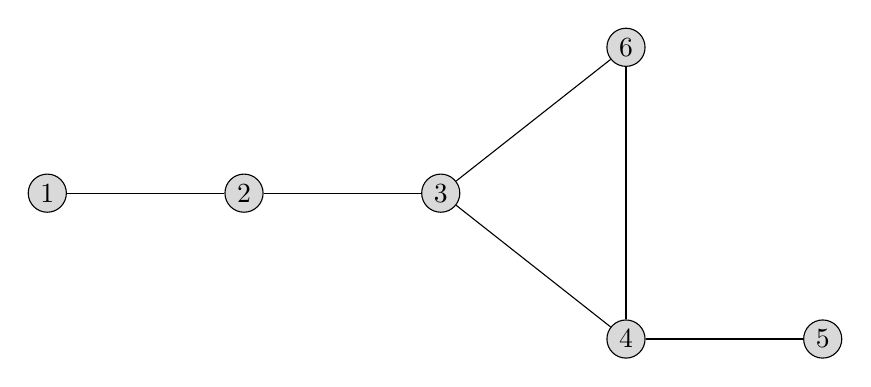
\begin{tikzpicture}[node distance=1.5cm and 2cm, auto, every node/.style={circle,draw,fill=gray!30,inner sep=2pt}]

% vertices
\node (1) {1};
\node (2) [right=of 1] {2};
\node (3) [right=of 2] {3};
\node (6) [above right=of 3] {6};
\node (4) [below right=of 3] {4};
\node (5) [right=of 4] {5};

% edges
\draw (1) -- (2);
\draw (2) -- (3);
\draw (3) -- (6);
\draw (3) -- (4);
\draw (6) -- (4);
\draw (4) -- (5);

\end{tikzpicture}

\subsection*{Question 10: Use the Cauchy-Frobenius-Burnside Theorem to determine the number of distinct
3-colourings of $C_8$.}

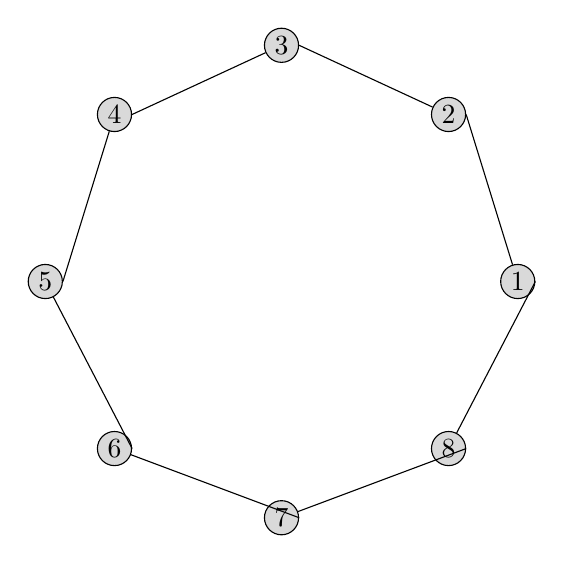
\begin{tikzpicture}[scale=3, every node/.style={circle, draw, fill=gray!30, inner sep=1.5pt}]

% Arrange 8 nodes evenly spaced on a circle
\foreach \i in {1,...,8} {
    \node (v\i) at ({360/8 * (\i - 1)}:1) {\i};
}

% Draw edges between consecutive vertices
\foreach \i [evaluate=\i as \next using {mod(\i,8) + 1}] in {1,...,8} {
    \draw (v\i) -- (v\next);
}

\end{tikzpicture}~\\
The automorphism group is the dihedral group, of order 16 (1 identity + 7 rotations + 8 reflections). There are $3^8$ 3-colourings. Each rotation fixes:
\begin{align*}
  1 &= 3 \text{ colourings } \\ 
  2 &= 3^2 = 9 \text{ colourings } \\ 
  3 &= 3 \text{ colourings } \\ 
  4 &= 3^4 = 81 \text{ colourings } \\ 
  5 &= 3 \text{ colourings } \\ 
  6 &= 3^2 = 9 \text{ colourings } \\ 
  7 &= 3 \text{ colourings } \\ 
\end{align*}
4 reflections fix $3^5$ colourings (reflections through vertices) and 4 reflections fix $3^4$ colourings (reflections through midpoints). So, by the Cauchy-Frobenius-Burnside theorem, there are: \[
\frac{1}{16} (3^8 + (3 + 9 + 3 + 81 + 3 + 9 + 3) + (4 \times 3^5 + 4 \times 3^4)) = 498
\]

\subsection*{Question 11: Use the Cauchy-Frobenius-Burnside Theorem to determine the number of graphs of order 5.}
\end{document}